\documentclass[12pt,a4paper]{article}

% Paquetes básicos
\usepackage[utf8]{inputenc}
\usepackage[T1]{fontenc}
\usepackage[spanish]{babel}
\usepackage{amsmath, amssymb}
\usepackage{siunitx} % Ángulos
\usepackage{graphicx}
\usepackage{float}
\usepackage{geometry}
\geometry{margin=2.5cm}
\usepackage{hyperref}
\usepackage{caption}
\usepackage{subcaption}
\usepackage{setspace}
\usepackage{multirow}
\usepackage{minted} % Códigos
\graphicspath{{Figuras/}}
\onehalfspacing


% Datos
\author{Nombre y Apellido \\ Legajo: XXXXX}
\date{\today}

\begin{document}

% Carátula personalizada
\begin{titlepage}
    \centering
    
\includegraphics[width=0.25\textwidth]{escudo.png} 
    \hspace{1cm}
    
\includegraphics[width=0.3\textwidth]{download.png} \\[1cm]

    {\large \textbf{UNIVERSIDAD NACIONAL DE CÓRDOBA} \\[0.5cm]}
    {\large \textbf {FACULTAD DE CIENCIAS EXACTAS, FÍSICAS Y NATURALES} \\[1cm]}
    {\Large ELECTRÓNICA INDUSTRIAL \\[1cm]}

    \rule{\textwidth}{0.5pt} \\[0.5cm]
    {\Large \textbf{Trabajo Práctico Teórico N°1} \\[0.3cm]}
    {\Large \textbf{Introducción a la Electrónica de Potencia} \\[0.3cm]}
    \rule{\textwidth}{0.5pt} \\[1cm]

\begin{tabular}{l l}
\textbf{Profesor Titular:} & Ing. Agüero Adrián.\\
\textbf{Profesor Adjunto:} & Ing. Gangi O. Sergio.\\
\textbf{Profesor Adjunto:} & Ing. Laboret Sergio.\\

\\
\textbf{Alumno:} Monja, Ernesto Joaquín. \\
\textbf{DNI:} 43.873.728 \\
\end{tabular}\\[3cm]

{\centering Año 2026 \par}

\end{titlepage}



% Índice
\tableofcontents
\newpage
\indent



\section{Introducción}
En este trabajo práctico se busca investigar sobre un sistema de potencia en donde se realice la conversión de energía de $AC$-$DC$-$DC$. Para ello, el sistema elegido es el sistema de conversión de potencia que ocurre para las herramientas eléctricas inalámbricas, tales como un taladro o un atornillador. Más específicamente estudiaremos sobre los taladros eléctricos inalámbricos y cómo se relacionan a los conceptos analizados en clase.


\section{Desarrollo}
\subsection{Consigna 1: Identificar Sistemas $AC$-$DC$-$DC$}
Como se mencionó anteriormente, el sistema de potencia elegido es un taladro eléctrico inalámbrico, ya que este contiene los procesos de conversión deseados:

\begin{itemize}
    \item \underline{Conversión $AC$-$DC$:} Se realiza esta conversión, esencialmente porque se debe rectificar la señal de entrada de la red a un valor de corriente continua, utilizando un puente de diodos tal como el que se muestra en la siguiente figura:
    \begin{figure}[H]
        \centering
        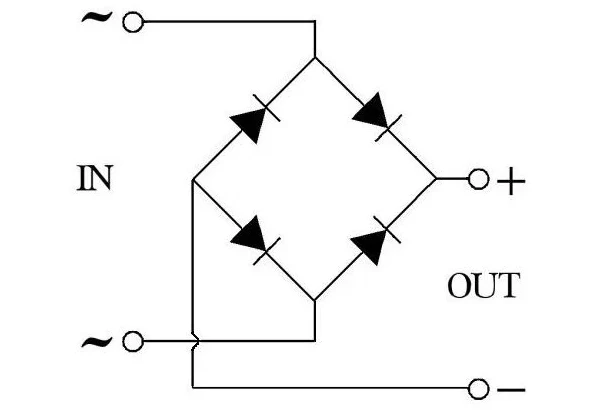
\includegraphics[width=0.5\linewidth]{Figura 1.png}
        \caption{\href{https://aragonelectronica.com/blogs/noticias/puente-de-diodo-2-0?srsltid=AfmBOorDnAsMsU1uF2HLmvZ3Y30DX13bp6w3tyW5yDUeuFGgX404lNbr}{Puente rectificador monofásico de diodos.}}
        \label{fig:fig_1}
    \end{figure}
    Aquí se trabaja con una tensión de entrada $V_{P} = 220/230 \ [V_{AC}]$ asumiendo que se trata de un taladro de uso doméstico y en consecuencia se conecta a una red monofásica, donde también debe notarse que en Argentina la frecuencia de la red es de $f = 50 \ [Hz]$. Se suelen trabajar con valores de salida de $V_{S} = 380/400 \ [V_{CC}]$ de modo que las corrientes de salida sean bajas para reducir la corriente y consecuentemente poder utilizar cables de menor sección por lo que se termina abaratando costos.
    
    \item \underline{Conversión $DC$-$DC$:} Se realiza esta conversión debido a que los taladros inalámbricos cuentan con baterías de CC, las cuales tienen valores de tensiones y corrientes muy específicos y controlados, tales como $12 \ [V]$, $18 \ [V]$ o $24 \ [V]$ mientras que la salida del rectificador es muy alta y no está regulada. Para ello se suelen usar Convertidores $DC$-$DC$ de tipo Flyback para el cual se presenta su circuito esquemático a continuación:
    \begin{figure}[H]
        \centering
        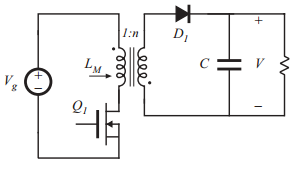
\includegraphics[width=0.4\linewidth]{Figura 2.png}
        \caption{{\href{https://electronics.stackexchange.com/questions/130766/flyback-converter-current-flow}{Circuito esquemático de un Convertidor Flyback.}}}
        \label{fig:fig_2}
    \end{figure}
    Muchos cargadores compactos utilizan los convertidores Flyback porque son baratos, requieren pocos componentes y proporcionan el aislamiento galvánico entre la red y la batería, que puede ser fundamental para proteger el circuito en caso de alguna falla. 
    Por lo general convertirán las tensiones y corrientes de salida del puente rectificador ($V_{S} = 380/400 \ [V_{CC}]$ e $I_{s} = 0,2/0,5 \ [A]$) en valores más comunes para una batería, tales como: $V_{o} = 18/20 \ [V]$ e $I_{o} = 2/4 \ [A]$.
\end{itemize}

Veamos finalmente el siguiente diagrama en bloques que esquematiza este proceso de conversión de potencia:

\begin{figure}[H]
    \centering
    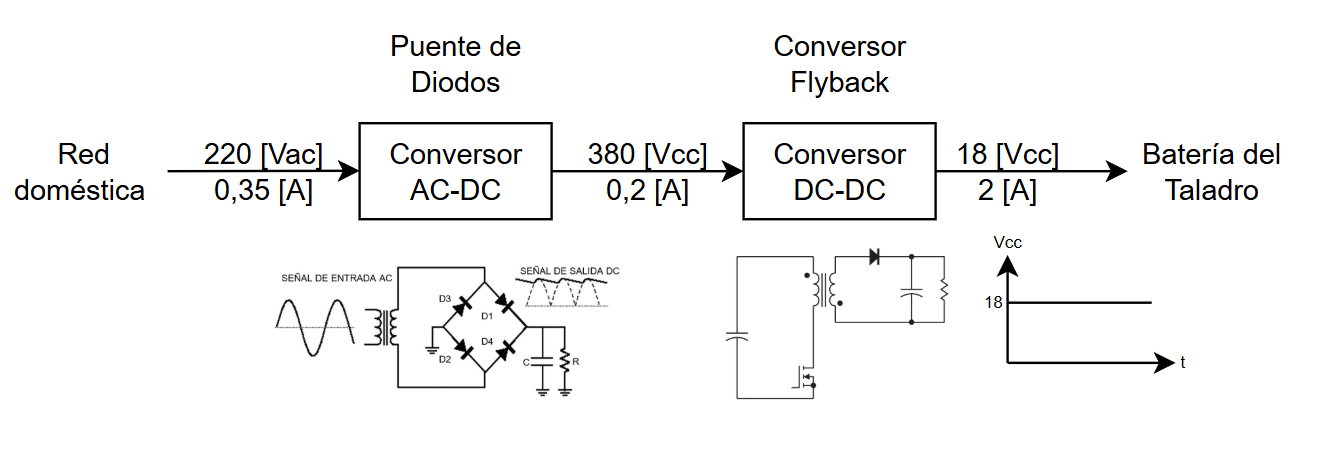
\includegraphics[width=1\linewidth]{Figura 3.png}
    \caption{Diagrama en bloques del Sistema de Potencia.}
    \label{fig:fig_3}
\end{figure}

Los valores de tensiones y corrientes mencionados son utilizados a modo de ejemplo y están elegidos en valores típicos de tensiones y corrientes para este tipo de circuito.



\subsection{Consigna 2: Especificaciones de Componentes}
La primera etapa contiene los diodos de rectificación de potencia, los cuales para un rectificador monofásico como es el caso de este taladro, se pueden utilizar los diodos 1N4007 los cuales en su hoja de datos, presentan la siguiente tabla:

\begin{figure}[H]
    \centering
    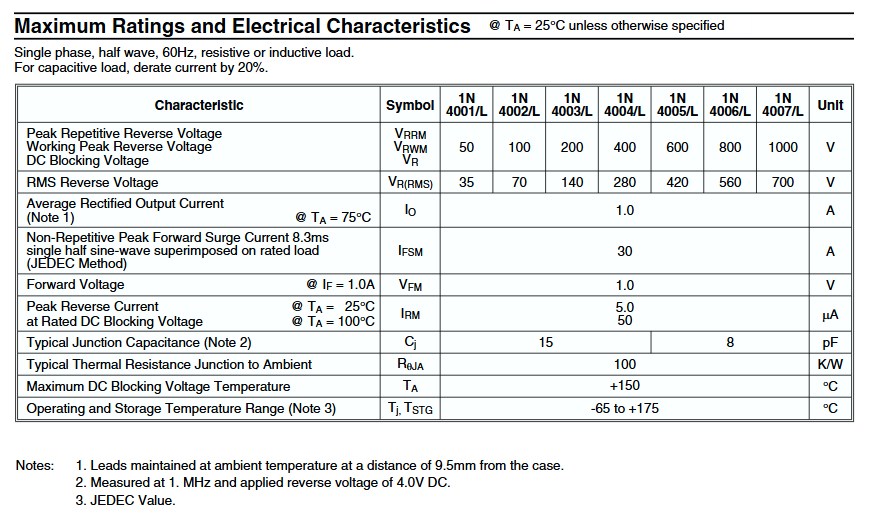
\includegraphics[width=0.77\linewidth]{Figura 4.png}
    \caption{\href{https://www.alldatasheet.com/datasheet-pdf/view/58830/DIODES/1N4007.html}{Características Eléctricas del Diodo 1N4007.}}
    \label{fig:fig_4}
\end{figure}

De aquí, resulta primordial definir los dos valores de preselección de un diodo, los cuales para nuestro modelo (1N4007), son:

\begin{itemize}
    \item \underline{Máxima Tensión Inversa Soportada:} En la hoja de datos, figura como: “Peak Repetitive Reverse Voltage” y es igual a: $V_{RRM} = 1000 \ [V]$
    \item \underline{Máxima Corriente Directa Conducida:} En la hoja de datos, figura como: “Non-Repetitive Peak Forward Surge Current 8.3ms single half sine-wave superimposed on rated load (JEDEC Method)” y es igual a: $I_{FSM} = 30 \ [A]$. El fabricante además incluye una gráfica que muestra la variación de esta corriente de acuerdo al número de ciclos:
    \begin{figure}[H]
        \centering
        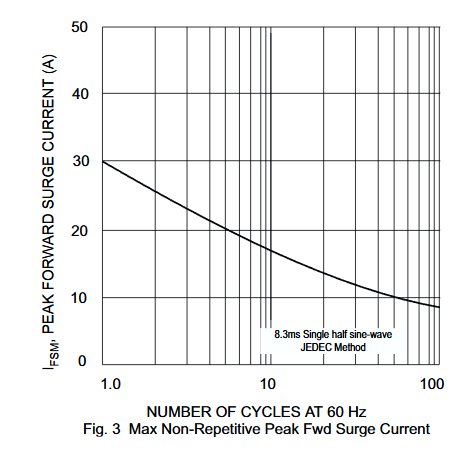
\includegraphics[width=0.4\linewidth]{Figura 5.png}
        \caption{Curva $I_{FSM}$-Numero de Ciclos}
        \label{fig:fig_5}
    \end{figure}
\end{itemize}

La hoja de datos incluye otros parámetros interesantes los cuales ya no se consideran de preselección, sino más bien parámetros ideales, los cuales pueden ser:

\begin{itemize}
    \item \underline{Caída de Tensión en Conducción:} Para ello, el fabricante nos provee una curva característica:
    \begin{figure}[H]
        \centering
        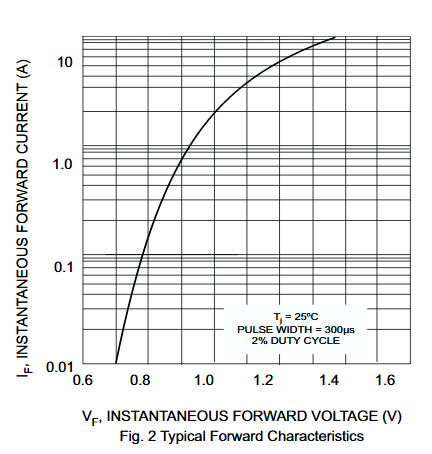
\includegraphics[width=0.4\linewidth]{Figura 6.png}
        \caption{Curva $I_{F}$-$V_{F}$}
        \label{fig:fig_6}
    \end{figure}
    \item \underline{Corriente Inversa de Bloqueo:} Se define en la Figura (\ref{fig:fig_4}) y se la encuentra como: “Peak Reverse Current at Rated DC Blocking Voltage” y es igual a: $I_{R} = 5/50 \ [\mu A]$ de acuerdo a la temperatura ambiente.
    \item \underline{Resistencia Térmica Juntura-Ambiente:} Si bien este encapsulado no permite la introducción de un disipador, es muy útil realizar el cálculo térmico del diodo. En este caso, el fabricante indica que: $R_{Th(JA)} = 100 \ [\frac{K}{W}]$
\end{itemize}

La segunda etapa de conversión ($DC$-$DC$), utiliza un convertidor Flyback el cual tiene en su interior un transistor MOSFET el cual tiene como función principal conectar y desconectar rápidamente el primario del transformador para poder transferir energía de forma controlada. Un ejemplo de estos transistores, puede ser el $IRF840$, el cual en su hoja de datos presenta una tabla con los siguientes valores:

\begin{figure}[H]
    \centering
    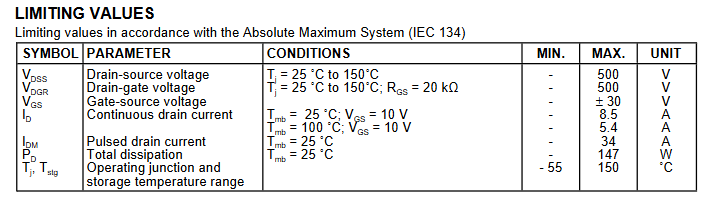
\includegraphics[width=0.9\linewidth]{Figura 7.png}
    \caption{\href{https://www.alldatasheet.com/datasheet-pdf/view/17804/PHILIPS/IRF840.html}{Características Eléctricas del MOSFET IRF840.}}
    \label{fig:fig_7}
\end{figure}

Se destacan los siguientes valores:

\begin{itemize}
    \item \underline{Tensión Drenador-Surtidor:} El convertidor Flyback genera picos de tensión los cuales debemos asegurar que el transistor pueda aguantar. En este caso, se tiene que: $V_{DS(max)} = 500 \ [V]$.
    \item \underline{Corriente de Drenador:} Se trata de la corriente máxima continua que puede conducir el transistor y se define como: $I_{D} = 8,5 \ [A]$.
    \item \underline{Potencia Disipada y Temperatura de Juntura:} Nos sirven para verificar si el mismo necesita o no un disipador. En este caso son iguales a: $P_{D} = 147 \ [W]$ y $T_{J} = 150 \ [°C]$.
\end{itemize}

También incluye una tabla como la siguiente:

\begin{figure}[H]
    \centering
    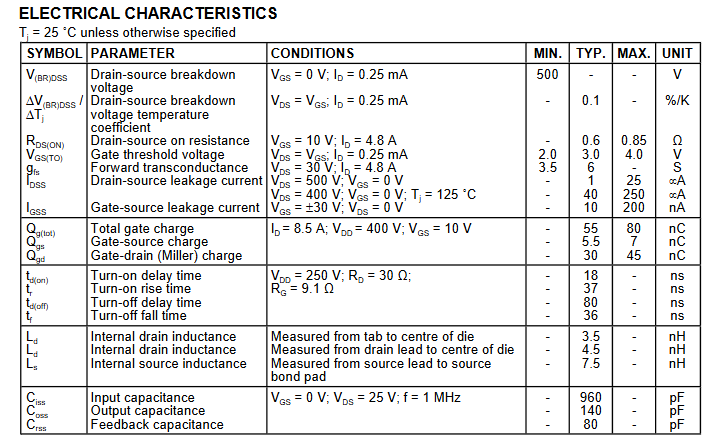
\includegraphics[width=0.9\linewidth]{Figura 8.png}
    \caption{\href{https://www.alldatasheet.com/datasheet-pdf/view/17804/PHILIPS/IRF840.html}{Características Eléctricas del MOSFET IRF840.}}
    \label{fig:fig_8}
\end{figure}

De aquí podemos destacar que los valores importantes para elegir el MOSFET pueden ser:

\begin{itemize}
    \item \underline{Resistencia Drenador-Surtidor Encendida:} Esta se trata de la resistencia interna del MOSFET cuando este se encuentra prendido y es la que nos permite calcular las pérdidas por conducción del MOSFET. En este caso, se tiene que: $R_{DS(ON)} = 0,6 \ [\Omega]$.
    \item \underline{Tiempos de respuesta:} En esta tabla, se incluyen tiempos de respuesta de delay, subida y caída para cuando el transistor conmuta y son útiles para diseñar el conmutador.
\end{itemize}



\subsection{Consigna 3: Simulación de Conmutación Ideal vs Real}
Para simular este ejercicio, se propuso realizar el siguiente circuito en LTSpice:

\begin{figure}[H]
    \centering
    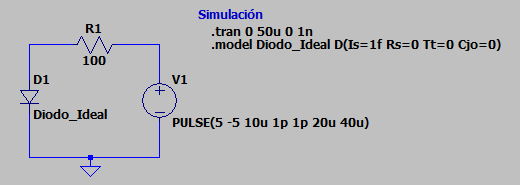
\includegraphics[width=0.6\linewidth]{Figura 9.png}
    \caption{Simulación en LTSpice de Circuito de Conmutación}
    \label{fig:fig_9}
\end{figure}

La idea consiste en simular una onda de tensión de pulsos, que varía de $5 \ [V]$ a $-5 \ [V]$ con unos parámetros de tiempo que se asimilen lo más posible a una fuente real (Específicamente el tiempo de subida y de bajada de la fuente al conmutar entre pulsos). La fuente conmuta en $10 \ [\mu s]$ y se queda por $20 \ [\mu s]$ en $-5 \ [V]$ para finalmente volver a $5 \ [V]$.

A continuación se presenta las formas de onda de Tensión, Corriente y Potencia a del diodo tras una conmutación ideal:

\begin{figure}[H]
    \centering
    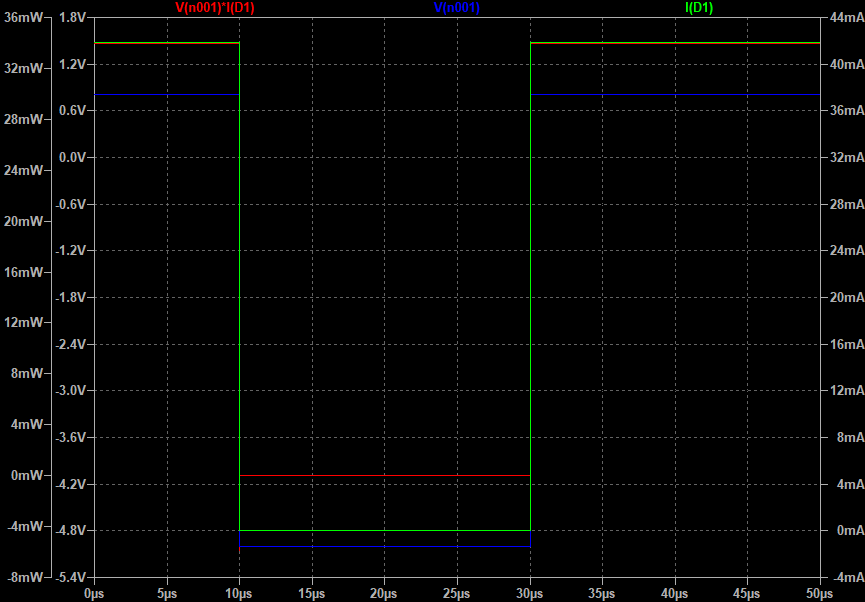
\includegraphics[width=1\linewidth]{Figura 10.png}
    \caption{Simulación en LTSpice de Circuito de Conmutación Ideal del Diodo.}
    \label{fig:fig_10}
\end{figure}

Cómo es de esperarse, no ocurren efectos transitorios sobre las formas de onda y estos actúan como se esperaría de un diodo ideal, tanto para tensión como para corriente y consecuentemente para la potencia siendo la multiplicación de estas dos anteriores.

Sin embargo veremos que esto no es lo mismo si se reemplaza el modelo del diodo ideal por un diodo real, como lo puede ser el 1N4007, donde ahora si ocurren efectos transitorios de la respuesta del diodo:

\begin{figure}[H]
    \centering
    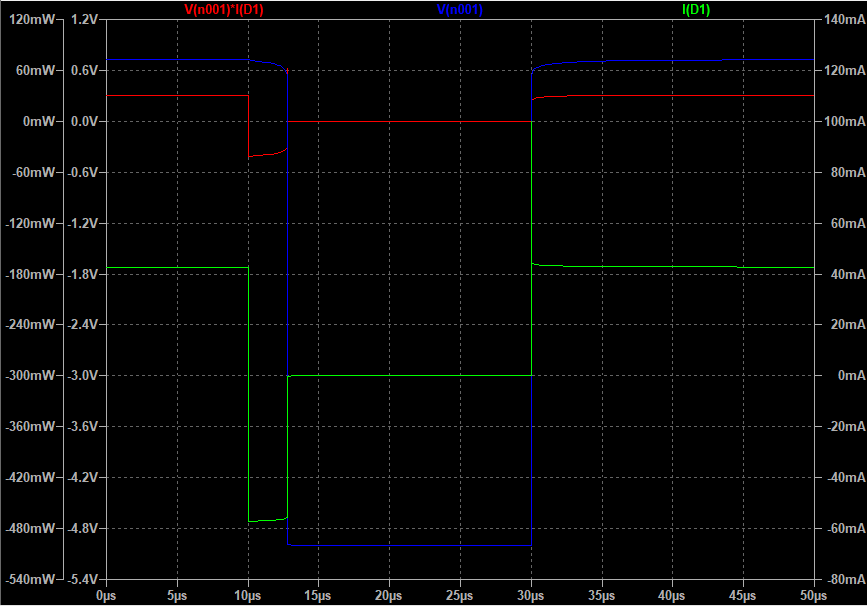
\includegraphics[width=1\linewidth]{Figura 11.png}
    \caption{Simulación en LTSpice de Circuito de Conmutación Real del Diodo.}
    \label{fig:fig_11}
\end{figure}

Aquí se ven justamente los efectos transitorios mencionados anteriormente que corresponden a un diodo real.



\subsection{Consigna 4: Análisis de un Sistema $DC$-$DC$-$AC$}
Un ejemplo claro de un sistema de potencia $DC$-$DC$-$AC$ es un sistema de UPS cuando ocurre un corte de energía como los estudiados en asignaturas como Instalaciones Eléctricas ya que:

\begin{itemize}
    \item \underline{Conversión $DC$-$DC$:} Al cortarse el suministro eléctrico de energía, se tiene que el rectificador deja de entregar energía y el sistema cambia a modo batería la cual suele ser de $12 \ [V]$, $24 \ [V]$ o $48 \ [V]$ sin embargo el inversor que convertirá la $DC$ a $AC$ necesita aproximadamente $320 \ [V_{DC}]$ para generar una tensión de $220 \ [V_{AC}]$ lo que implica que se necesitará un Convertidor Push-Pull el cual tiene la siguiente topología:
    \begin{figure}[H]
        \centering
        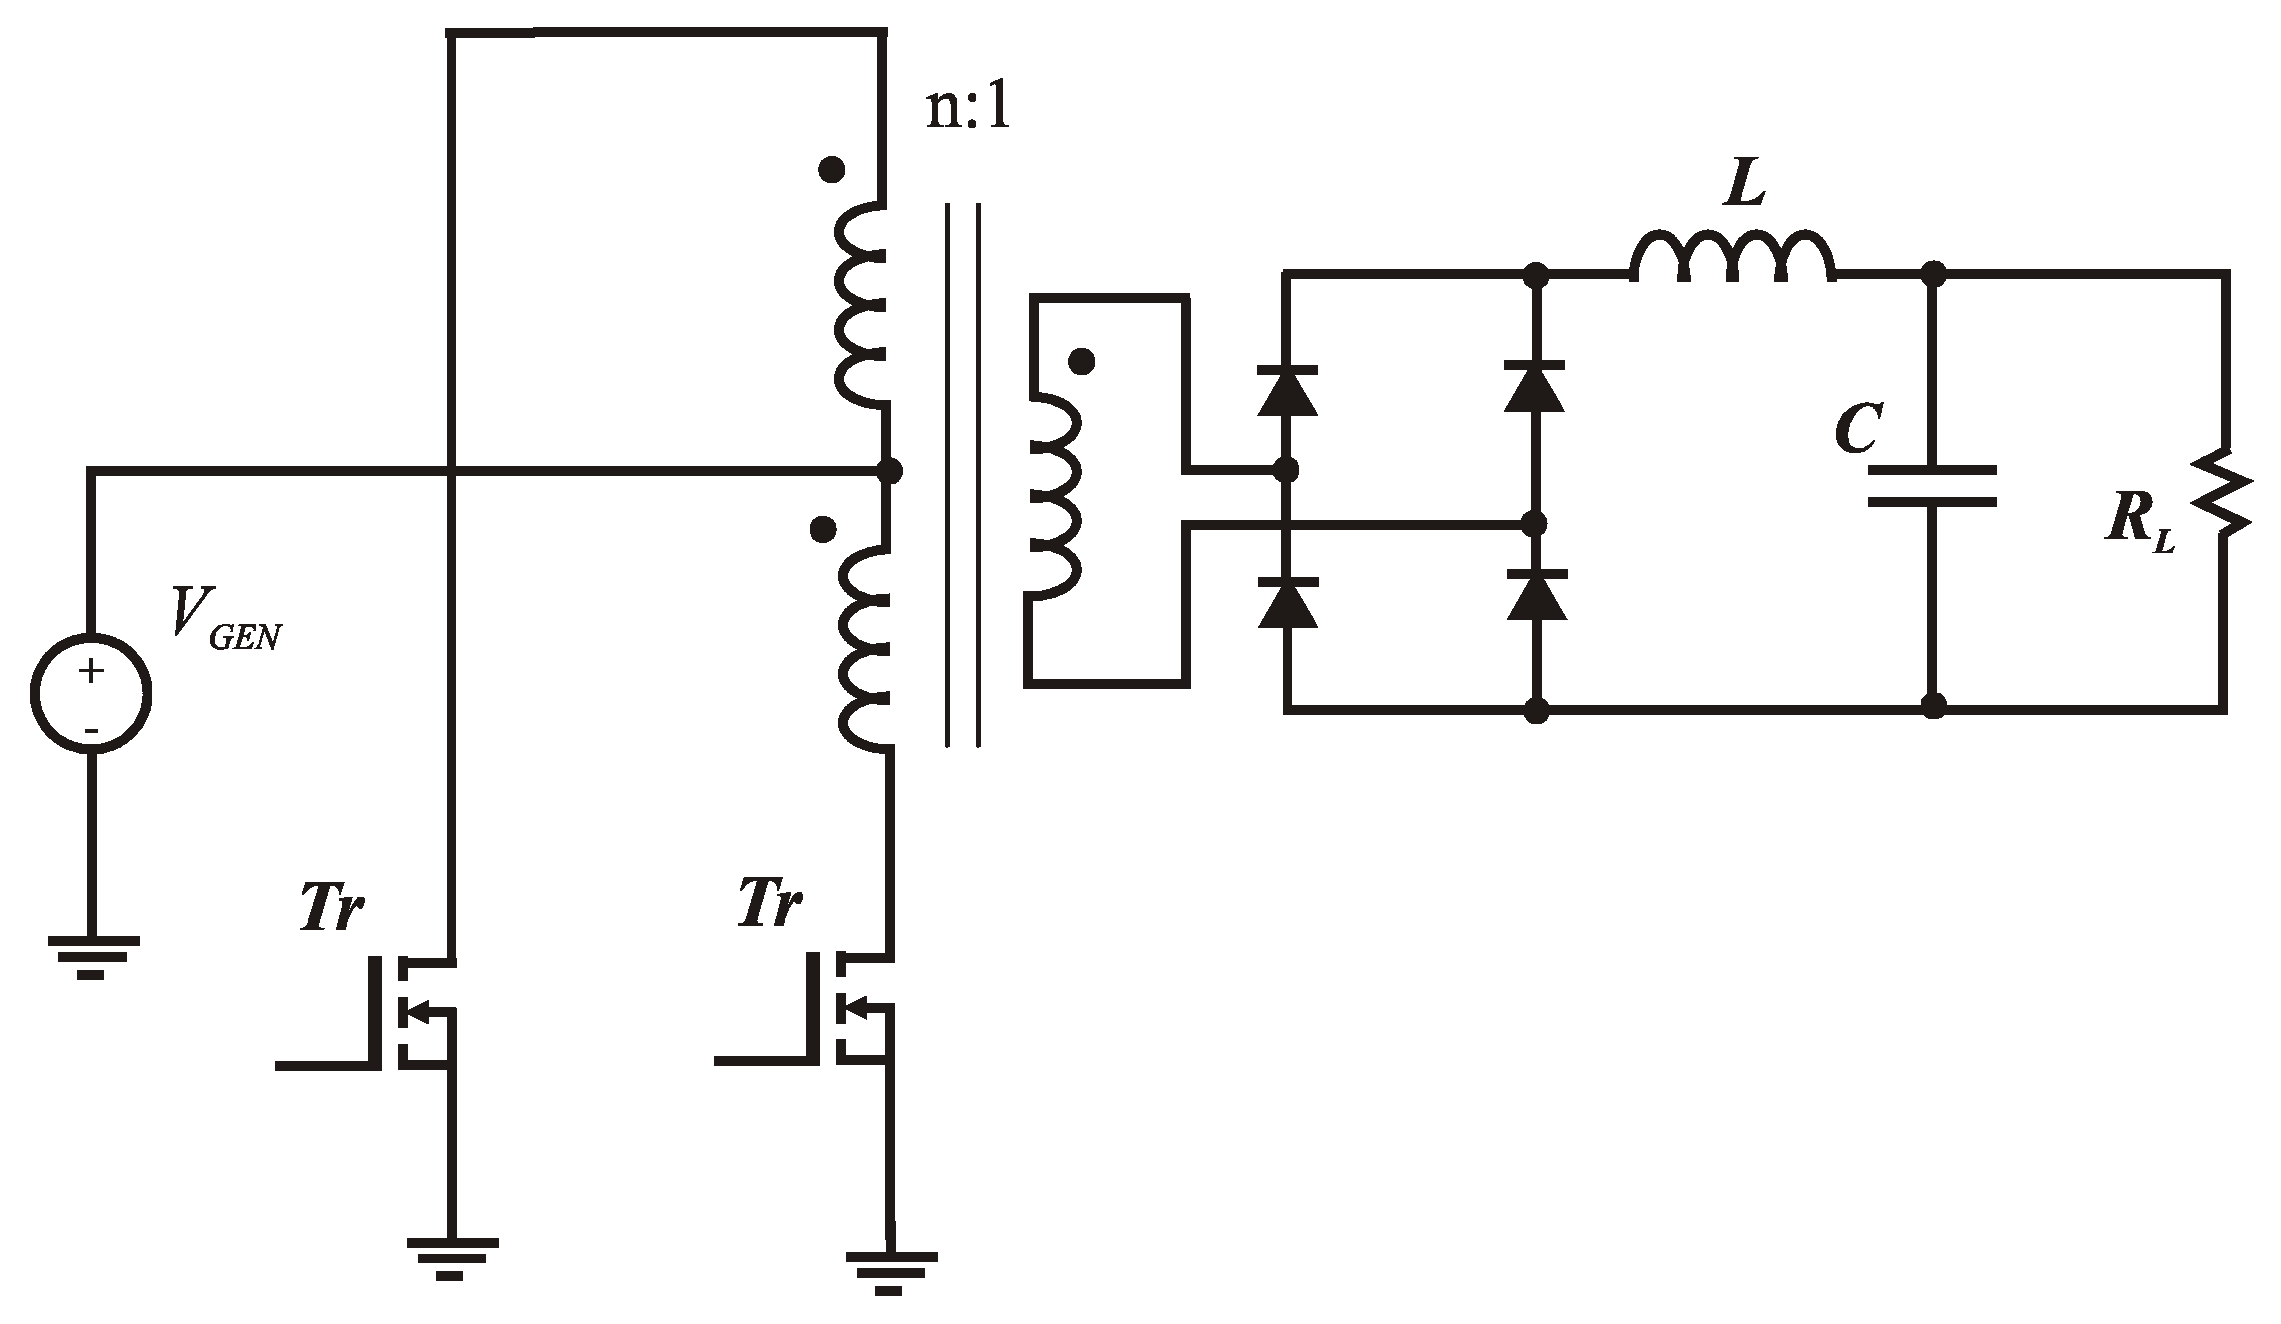
\includegraphics[width=0.6\linewidth]{Figura 12.png}
        \caption{\href{https://www.mdpi.com/2079-9292/11/17/2713}{Circuito Esquemático de un Convertidor de Push-Pull.}}
        \label{fig:fig_12}
    \end{figure}
    Se utilizan convertidores con transformadores dada la facilidad que se tiene para elevar la tensión dada una relación de espiras.

    \item \underline{Conversión $DC$-$AC$:} La idea consiste en convertir esta señal de DC elevada en una continua la cual pasará por muchas etapas para primero lograr alternarla, luego generar un efecto sinusoidal y finalmente suavizarla. Para la primera parte, se usa un Puente H como el que se muestra en la siguiente figura:
    \begin{figure}[H]
        \centering
        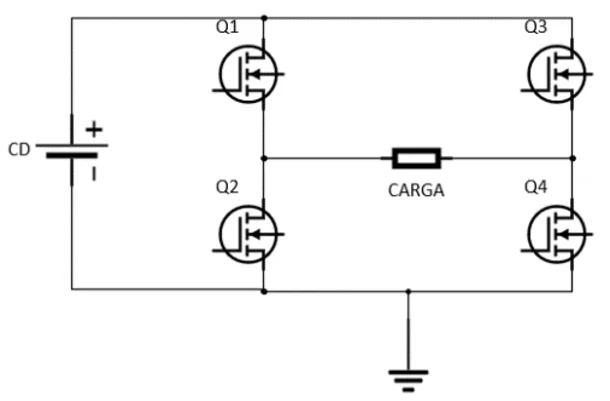
\includegraphics[width=0.5\linewidth]{Figuras/Figura 13.png}
        \caption{\href{https://scielo.conicyt.cl/pdf/formuniv/v9n1/art13.pdf}{Circuito esquemático del Puente H.}}
        \label{fig:fig_13}
    \end{figure}
    Este puente, nos permitirá pasar de una señal de $DC$ a una señal de pulsos cuadrados, los cuales luego pasaran por un modulador PWM que les dará una forma sinusoidal y se terminarán de suavizar con un filtro LC.
\end{itemize}

Se presenta a continuación un diagrama en bloques que esquematiza el proceso de conversión de potencia:

\begin{figure}[H]
    \centering
    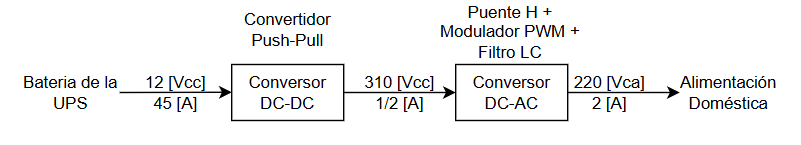
\includegraphics[width=1\linewidth]{Figuras/Figura 14.png}
    \caption{Diagrama en bloques del Sistema de Potencia.}
    \label{fig:fig_14}
\end{figure}

Los valores de tensiones y corrientes mencionados son utilizados a modo de ejemplo y están elegidos en valores típicos de tensiones y corrientes para este tipo de circuito.

Finalmente, se puede analizar los componentes de potencia de estas etapas, sin embargo vemos que tanto este sistema de potencia como el sistema analizado en la Figura (\ref{fig:fig_3}), están compuestos por transistores MOSFETS y Diodos Rectificadores, por lo tanto se resumirá la explicación de la búsqueda de datos eléctricos de los mismos ya que estos ya fueron explicados en la Subsección 2.2 de este informe.

Partamos por el conversor $DC$-$DC$, más específicamente por los diodos utilizados en el Convertidor Push-Pull, los cuales se eligen fundamentalmente en base a la Máxima Tensión Inversa Soportada y Máxima Corriente Directa Conducida. Nótese que para este tipo de aplicaciones, un diodo 1N4007 se quemaría dadas las altas frecuencias, por lo tanto se debe elegir un diodo como el MUR460 el cual según su hoja de datos, presenta la siguiente tabla:

\begin{figure}[H]
    \centering
    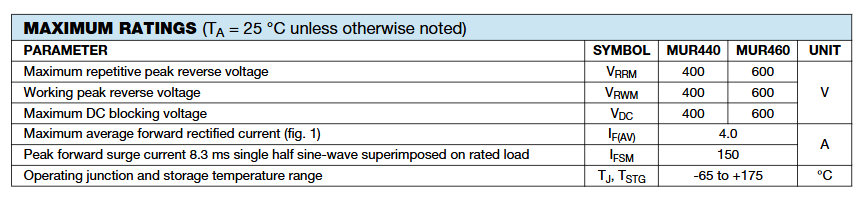
\includegraphics[width=1\linewidth]{Figuras/Figura 15.png}
    \caption{\href{https://www.alldatasheet.com/datasheet-pdf/view/1397411/VISHAY/MUR460.html}{Características Eléctricas del Diodo MUR460.}}
    \label{fig:fig_15}
\end{figure}

De aquí se deduce fácilmente que:
\begin{itemize}
    \item \underline{Máxima Tensión Inversa Soportada:} $V_{RRM} = 600 \ [V]$.
    \item \underline{Máxima Corriente Directa Conducida:} $I_{FSM} = 150 \ [A]$.
\end{itemize}

Luego, para el conversor $DC$-$AC$, podemos ver los MOSFETs de potencia utilizados en el Puente H, para los cuales se suelen utilizar los STW20NM60 los cuales tienen en su hoja de datos los siguientes valores:

\begin{figure}[H]
    \centering
    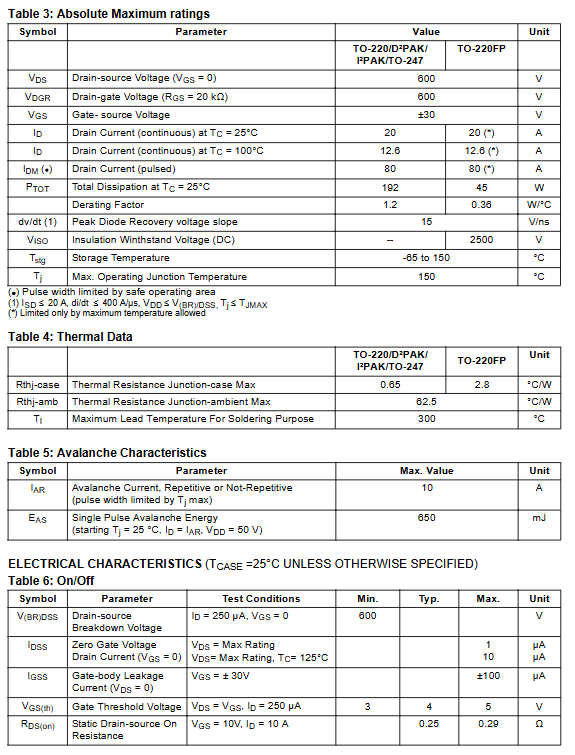
\includegraphics[width=0.8\linewidth]{Figuras/Figura 16.png}
    \caption{\href{https://www.alldatasheet.com/datasheet-pdf/view/24354/STMICROELECTRONICS/STW20NM60.html}{Características Eléctricas del MOSFET STW20NM60.}}
    \label{fig:fig_16}
\end{figure}

De aquí se deduce fácilmente que:
\begin{itemize}
    \item \underline{Tensión Drenador-Surtidor:} $V_{DS} = 600 \ [V]$.
    \item \underline{Corriente de Drenador:} $I_{FSM} = 20 \ [A]$ a $T = 25 \ [°C]$.
    \item \underline{Potencia Disipada y Temperatura de Juntura:} $P_D = 192 \ [W]$ para el encapsulado TO-220.
    \item \underline{Resistencia Drenador-Surtidor Encendida:} $R_{DS(on)} = 0,25 \ [\Omega]$
\end{itemize}


\section{Conclusiones}
A lo largo de este informe, se ha investigado 2 sistemas de conversión de potencia en cuanto a su funcionamiento, valores típicos de tensión y corriente, y se buscaron datos útiles de hojas de datos de componentes de potencia de cada etapa conversora de potencia, para seleccionar correctamente un componente. Así mismo se realizó una simulación sobre las conmutaciones ideales y reales de un diodo y sus efectos en las tensiones, corrientes y potencia del diodo.

\end{document}